\documentclass[11pt]{article}

\usepackage{fontspec}
\setmainfont{Times New Roman}
\usepackage[a4paper,margin=2.4cm]{geometry}
\usepackage{amsmath,amssymb}
\usepackage{graphicx}
\usepackage{float}
\usepackage{booktabs}
\usepackage{caption}
\usepackage{xcolor}
\usepackage[hidelinks]{hyperref}

\captionsetup{font=small,labelfont=bf}
\renewcommand{\abstractname}{Аннотация}
\setlength{\parindent}{0pt}
\setlength{\parskip}{0.55em}

\title{\textbf{Система Лоренца}\\[0.25em]
\large численное решение, устойчивость и хаос}
\author{Отчёт подготовлен в DeepSeek Harness\\с плагином \texttt{dsh-wolfram-nb} (Wolfram Language)}
\date{12 ноября 2026}

\begin{document}
\maketitle

\begin{abstract}
Рассмотрена классическая нелинейная система Лоренца. Найдены точки равновесия и исследована их
устойчивость, численно решена задача Коши на отрезке $t\in[0,40]$, построены двумерные и
трёхмерные графики, а также количественно показана чувствительность решения к начальным данным:
расхождение двух траекторий растёт экспоненциально с показателем $\lambda\approx0.88$,
что согласуется с известным старшим ляпуновским показателем системы ($\approx0.906$).
\end{abstract}

\section{Постановка задачи}

Система Лоренца имеет вид
\begin{equation}
\dot{x}=\sigma\,(y-x),\qquad
\dot{y}=x\,(\rho-z)-y,\qquad
\dot{z}=x\,y-\beta\,z,
\label{eq:lorenz}
\end{equation}
где $\sigma,\rho,\beta>0$ --- параметры. В работе используются классические значения
\[
\sigma=10,\qquad \rho=28,\qquad \beta=\frac{8}{3},
\]
при которых система демонстрирует детерминированный хаос.

Задача Коши ставится с начальными условиями
\[
x(0)=1,\qquad y(0)=1,\qquad z(0)=1,
\]
а для исследования чувствительности --- ещё с одним набором
\[
x_2(0)=1.001,\qquad y_2(0)=1,\qquad z_2(0)=1,
\]
отличающимся от первого только на $10^{-3}$ по координате $x$.

\section{Точки равновесия и их устойчивость}

\subsection{Положения равновесия}

Приравнивая правые части \eqref{eq:lorenz} к нулю, из первого уравнения получаем $y=x$,
из второго --- $x(\rho-z)=y=x$, откуда $z=\rho-1$ при $x\ne0$. Третье уравнение даёт
$x^{2}=\beta(\rho-1)$. Итак, имеются три точки равновесия:
\[
O=(0,0,0),\qquad
C_{\pm}=\bigl(\pm r,\ \pm r,\ \rho-1\bigr),
\qquad r=\sqrt{\beta(\rho-1)}.
\]
Для выбранных параметров
\[
r=\sqrt{\tfrac{8}{3}\cdot 27}=\sqrt{72}=6\sqrt{2}\approx 8.4853,
\qquad \rho-1=27.
\]
Таким образом,
\[
O=(0,0,0),\qquad
C_{+}\approx(8.4853,\ 8.4853,\ 27),\qquad
C_{-}\approx(-8.4853,\ -8.4853,\ 27).
\]

\subsection{Линеаризация}

Матрица Якоби системы \eqref{eq:lorenz}:
\begin{equation}
J(x,y,z)=
\begin{pmatrix}
-\sigma & \sigma & 0\\
\rho-z & -1 & -x\\
y & x & -\beta
\end{pmatrix}.
\label{eq:jac}
\end{equation}

\paragraph{Точка $O$.}
При $(x,y,z)=(0,0,0)$
\[
J(O)=\begin{pmatrix}-10&10&0\\ 28&-1&0\\ 0&0&-\tfrac83\end{pmatrix},
\]
её собственные значения
\[
\lambda_1\approx-22.8277,\qquad
\lambda_2\approx-2.6667,\qquad
\lambda_3\approx 11.8277.
\]
Одно собственное значение положительно, поэтому $O$ --- \emph{седло}: неустойчивая точка.

\paragraph{Точки $C_{\pm}$.}
При $(x,y,z)=(\pm r,\pm r,27)$ собственные значения одинаковы для обеих точек:
\[
\lambda_1\approx-13.8546,\qquad
\lambda_{2,3}\approx 0.0940\pm 10.1945\,i.
\]
Вещественная часть комплексной пары положительна, следовательно $C_{\pm}$ ---
\emph{неустойчивые седло-фокусы}. Все три равновесия неустойчивы, и траектория вынуждена
блуждать в ограниченной области --- это и есть странный аттрактор Лоренца.

\section{Численное решение}

Задача Коши решалась методом Рунге---Кутты с адаптивным шагом (функция \texttt{NDSolve}
Wolfram Language) на отрезке $t\in[0,40]$:
{\small
\begin{verbatim}
lorenz = NDSolve[{x'[t] == 10 (y[t] - x[t]),
                  y'[t] == x[t] (28 - z[t]) - y[t],
                  z'[t] == x[t] y[t] - 8/3 z[t],
                  x[0] == 1, y[0] == 1, z[0] == 1},
                 {x, y, z}, {t, 0, 40}, MaxSteps -> Infinity];
\end{verbatim}
}
Вторая траектория вычислялась тем же кодом с $x_2(0)=1.001$.

В момент $t=40$ первая траектория находится в точке
\[
\bigl(x(40),\,y(40),\,z(40)\bigr)\approx(-1.9656,\ -0.1696,\ 23.2846).
\]

\section{Чувствительность к начальным данным}

Пусть
\[
\Delta(t)=\bigl\|\mathbf{u}(t)-\mathbf{u}_2(t)\bigr\|,
\qquad \mathbf{u}=(x,y,z).
\]
В начальный момент $\Delta(0)=10^{-3}$. Значения расхождения приведены в таблице~\ref{tab:delta}.

\begin{table}[h]
\centering
\caption{Расхождение двух траекторий.}
\label{tab:delta}
\begin{tabular}{rcccccccc}
\toprule
$t$ & 5 & 10 & 15 & 20 & 25 & 30 & 35 & 40\\
\midrule
$\Delta(t)$ & 0.00125 & 0.00177 & 0.0233 & 0.911 & 6.40 & 17.6 & 14.6 & 20.8\\
\bottomrule
\end{tabular}
\end{table}

На участке экспоненциального роста расхождение аппроксимировалось моделью
\[
\ln\Delta(t)\approx \lambda t+c.
\]
Метод наименьших квадратов на отрезке $t\in[12,18]$ даёт
\[
\lambda\approx 0.880,\qquad R^{2}\approx 0.751,
\]
что близко к известному старшему ляпуновскому показателю системы Лоренца
$\lambda_{\max}\approx0.906$. Оценка снизу занижена из-за конечной длины ряда и насыщения
расхождения на масштабе аттрактора.

Расхождение достигает единицы (порядка размера аттрактора) уже при
\[
t_{1}\approx 18.33,
\]
то есть за время порядка $1/\lambda$ точность предсказания теряется полностью.

\section{Результаты}

На рис.~\ref{fig:time} показаны временные зависимости координат, на рис.~\ref{fig:xy} ---
проекция траектории на плоскость $x$--$y$, на рис.~\ref{fig:3d} --- трёхмерный аттрактор,
на рис.~\ref{fig:div} --- рост расхождения $\Delta(t)$ в логарифмическом масштабе.

\begin{figure}[H]
\centering
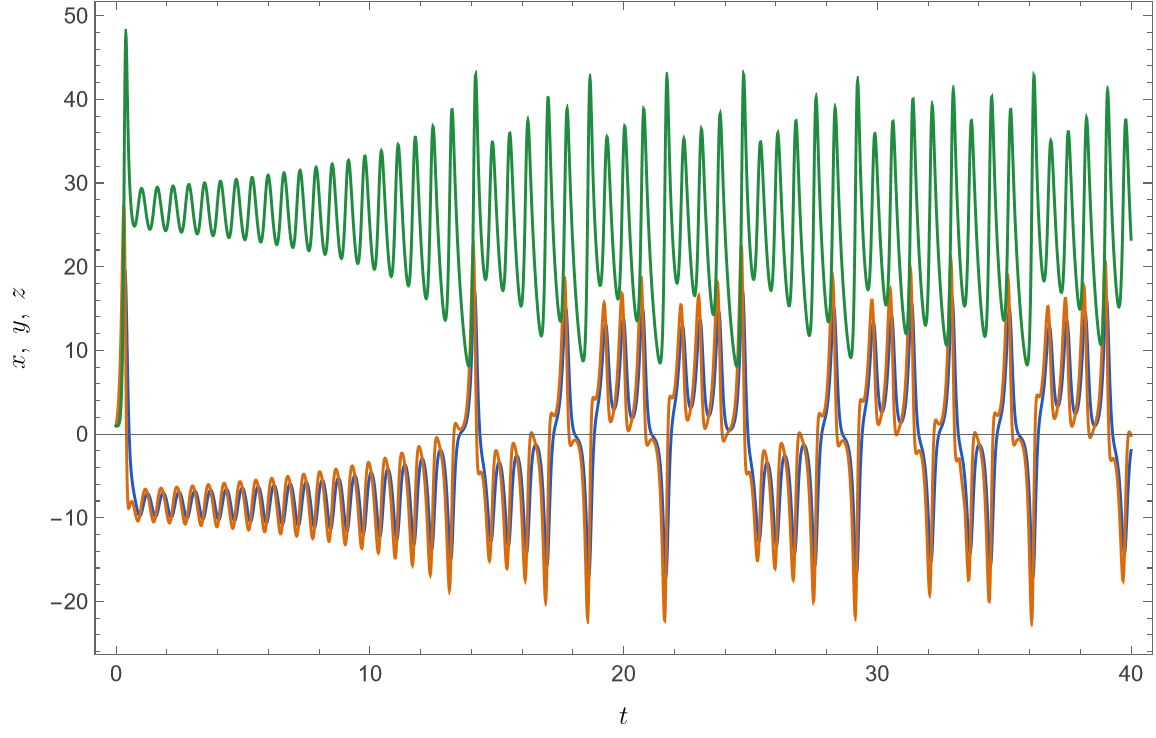
\includegraphics[width=0.78\textwidth]{_plots/lorenz-time.png}
\caption{Координаты $x(t)$, $y(t)$, $z(t)$ на отрезке $t\in[0,40]$.}
\label{fig:time}
\end{figure}

\begin{figure}[H]
\centering
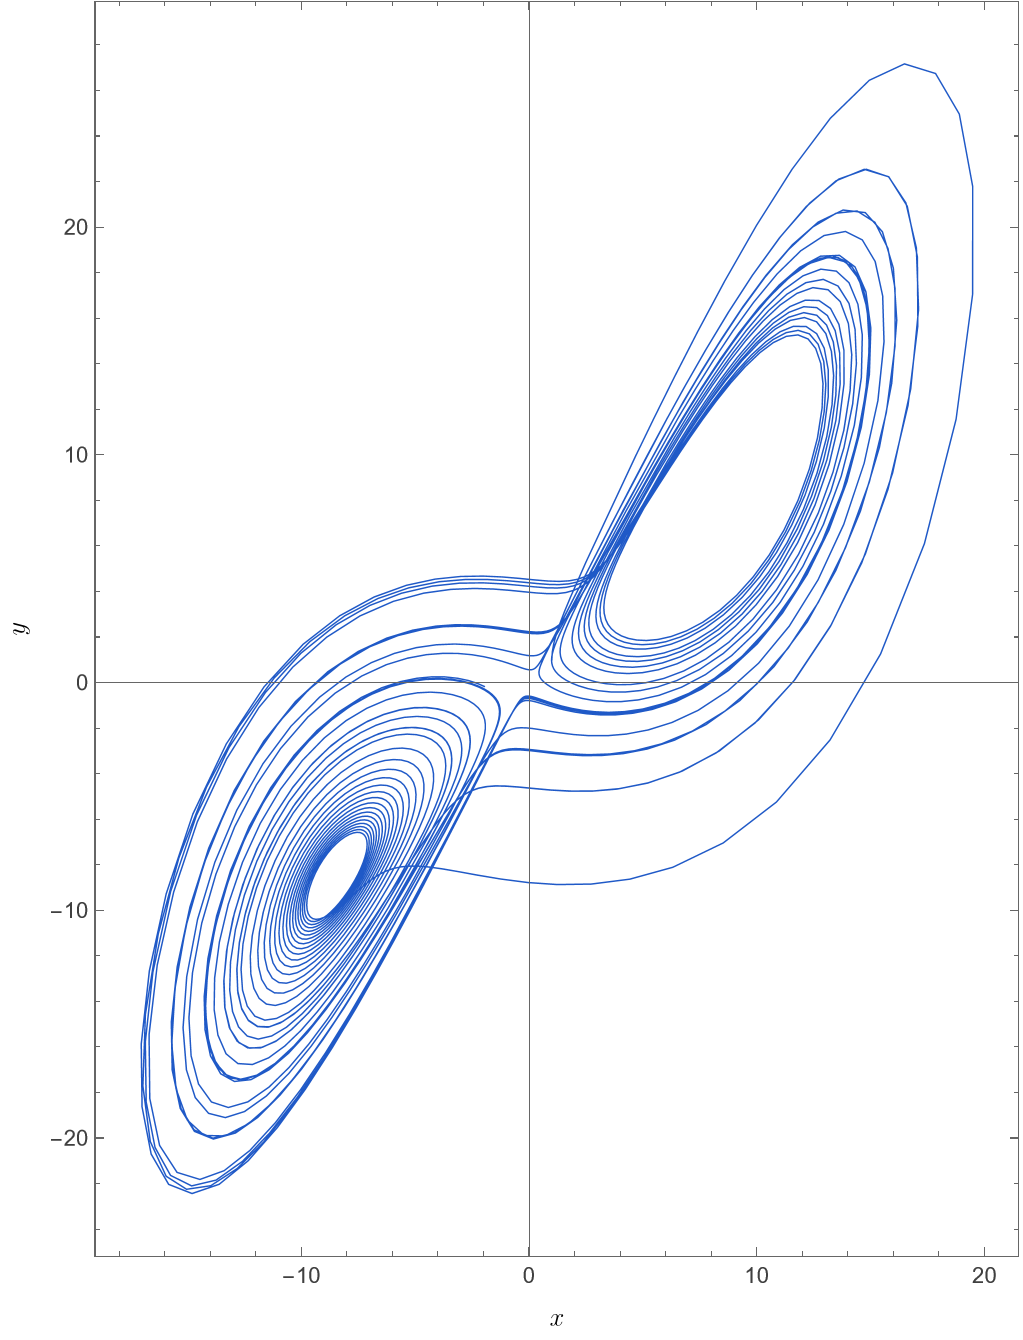
\includegraphics[width=0.42\textwidth]{_plots/lorenz-xy.png}
\caption{Проекция аттрактора на плоскость $x$--$y$.}
\label{fig:xy}
\end{figure}

\begin{figure}[H]
\centering
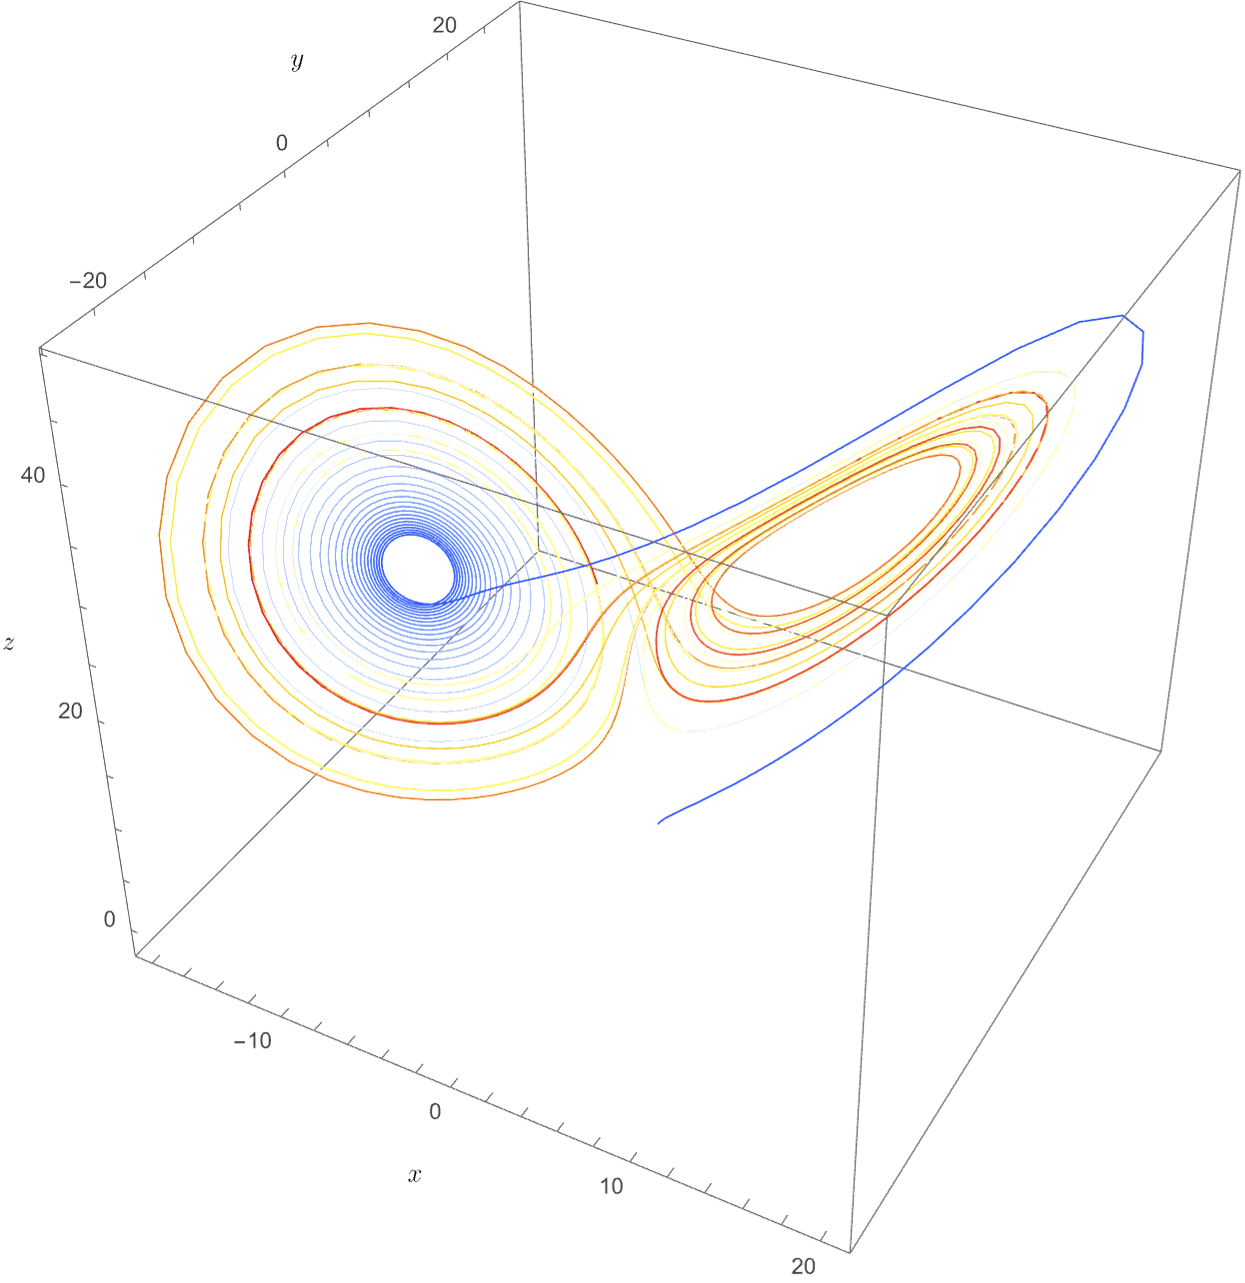
\includegraphics[width=0.60\textwidth]{_plots/lorenz-3d.png}
\caption{Трёхмерный аттрактор Лоренца; цвет --- время.}
\label{fig:3d}
\end{figure}

\begin{figure}[H]
\centering
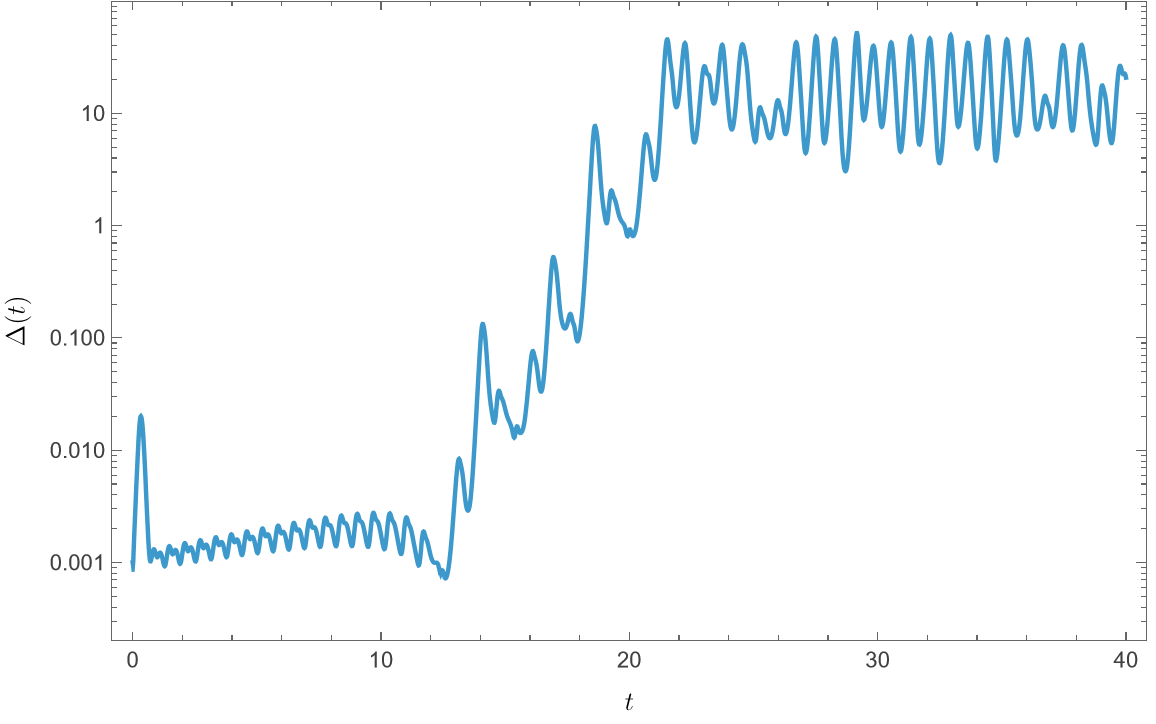
\includegraphics[width=0.68\textwidth]{_plots/lorenz-divergence.png}
\caption{Рост расстояния между двумя траекториями с начальной разницей $10^{-3}$.}
\label{fig:div}
\end{figure}

\section{Выводы}

\begin{enumerate}
\item У системы Лоренца при $\sigma=10$, $\rho=28$, $\beta=8/3$ три неустойчивых равновесия:
седло в начале координат и два седло-фокуса $C_{\pm}$.
\item Численное решение задачи Коши демонстрирует хаотическое поведение: траектория
навивается на аттрактор, не повторяясь.
\item Малое возмущение начальных данных ($10^{-3}$) приводит к расхождению траекторий
до порядка размера аттрактора за $t\approx 18$.
\item Оценка старшего ляпуновского показателя по расхождению, $\lambda\approx0.88$,
согласуется с литературным значением $\lambda_{\max}\approx0.906$.
\end{enumerate}

\end{document}
